\documentclass[11pt]{article}
\usepackage{geometry} % Pour passer au format A4
\geometry{hmargin=1cm, vmargin=1cm} % 

% Page et encodage
\usepackage[T1]{fontenc} % Use 8-bit encoding that has 256 glyphs
\usepackage[english,french]{babel} % Français et anglais
\usepackage[utf8]{inputenc} 

\usepackage{lmodern}
\setlength\parindent{0pt}

% Graphiques
\usepackage{graphicx,float,grffile}

% Maths et divers
\usepackage{amsmath,amsfonts,amssymb,amsthm,verbatim}
\usepackage{multicol,enumitem,url,eurosym,gensymb}

% Sections
\usepackage{sectsty} % Allows customizing section commands
\allsectionsfont{\centering \normalfont\scshape}

% Tête et pied de page

\usepackage{fancyhdr} 
\pagestyle{fancyplain} 

\fancyhead{} % No page header
\fancyfoot{}

\renewcommand{\headrulewidth}{0pt} % Remove header underlines
\renewcommand{\footrulewidth}{0pt} % Remove footer underlines

\newcommand{\horrule}[1]{\rule{\linewidth}{#1}} % Create horizontal rule command with 1 argument of height

%----------------------------------------------------------------------------------------
%	Début du document
%----------------------------------------------------------------------------------------

\begin{document}

%----------------------------------------------------------------------------------------
% RE-DEFINITION
%----------------------------------------------------------------------------------------
% MATHS
%-----------

\newtheorem{Definition}{Définition}
\newtheorem{Theorem}{Théorème}
\newtheorem{Proposition}{Propriété}

% MATHS
%-----------
\renewcommand{\labelitemi}{$\bullet$}
\renewcommand{\labelitemii}{$\circ$}
%----------------------------------------------------------------------------------------
%	Titre
%----------------------------------------------------------------------------------------

\setlength{\columnseprule}{0pt}

\section*{DM - TRI3 - DM1}
\textit{Pour le 25/03}
\horrule{2px} 

\begin{multicols}{2}

\subsection*{EX1 - CORRECTION}
\textit{\textbf{Recopier à l'identique la correction de l'exercice 1 du brevet blanc.}}

\begin{itemize}
	\item[A.a)] Calcul de l'étendu : max - min.\\
	étendue = 48 - 30 = 18\\
	L'étendu de la série de récoltes est 18kg.
	\item[A.b)] On compte 25 carreaux. La médiane est la 13è valeur. 
	\begin{figure}[H]
		\centering
		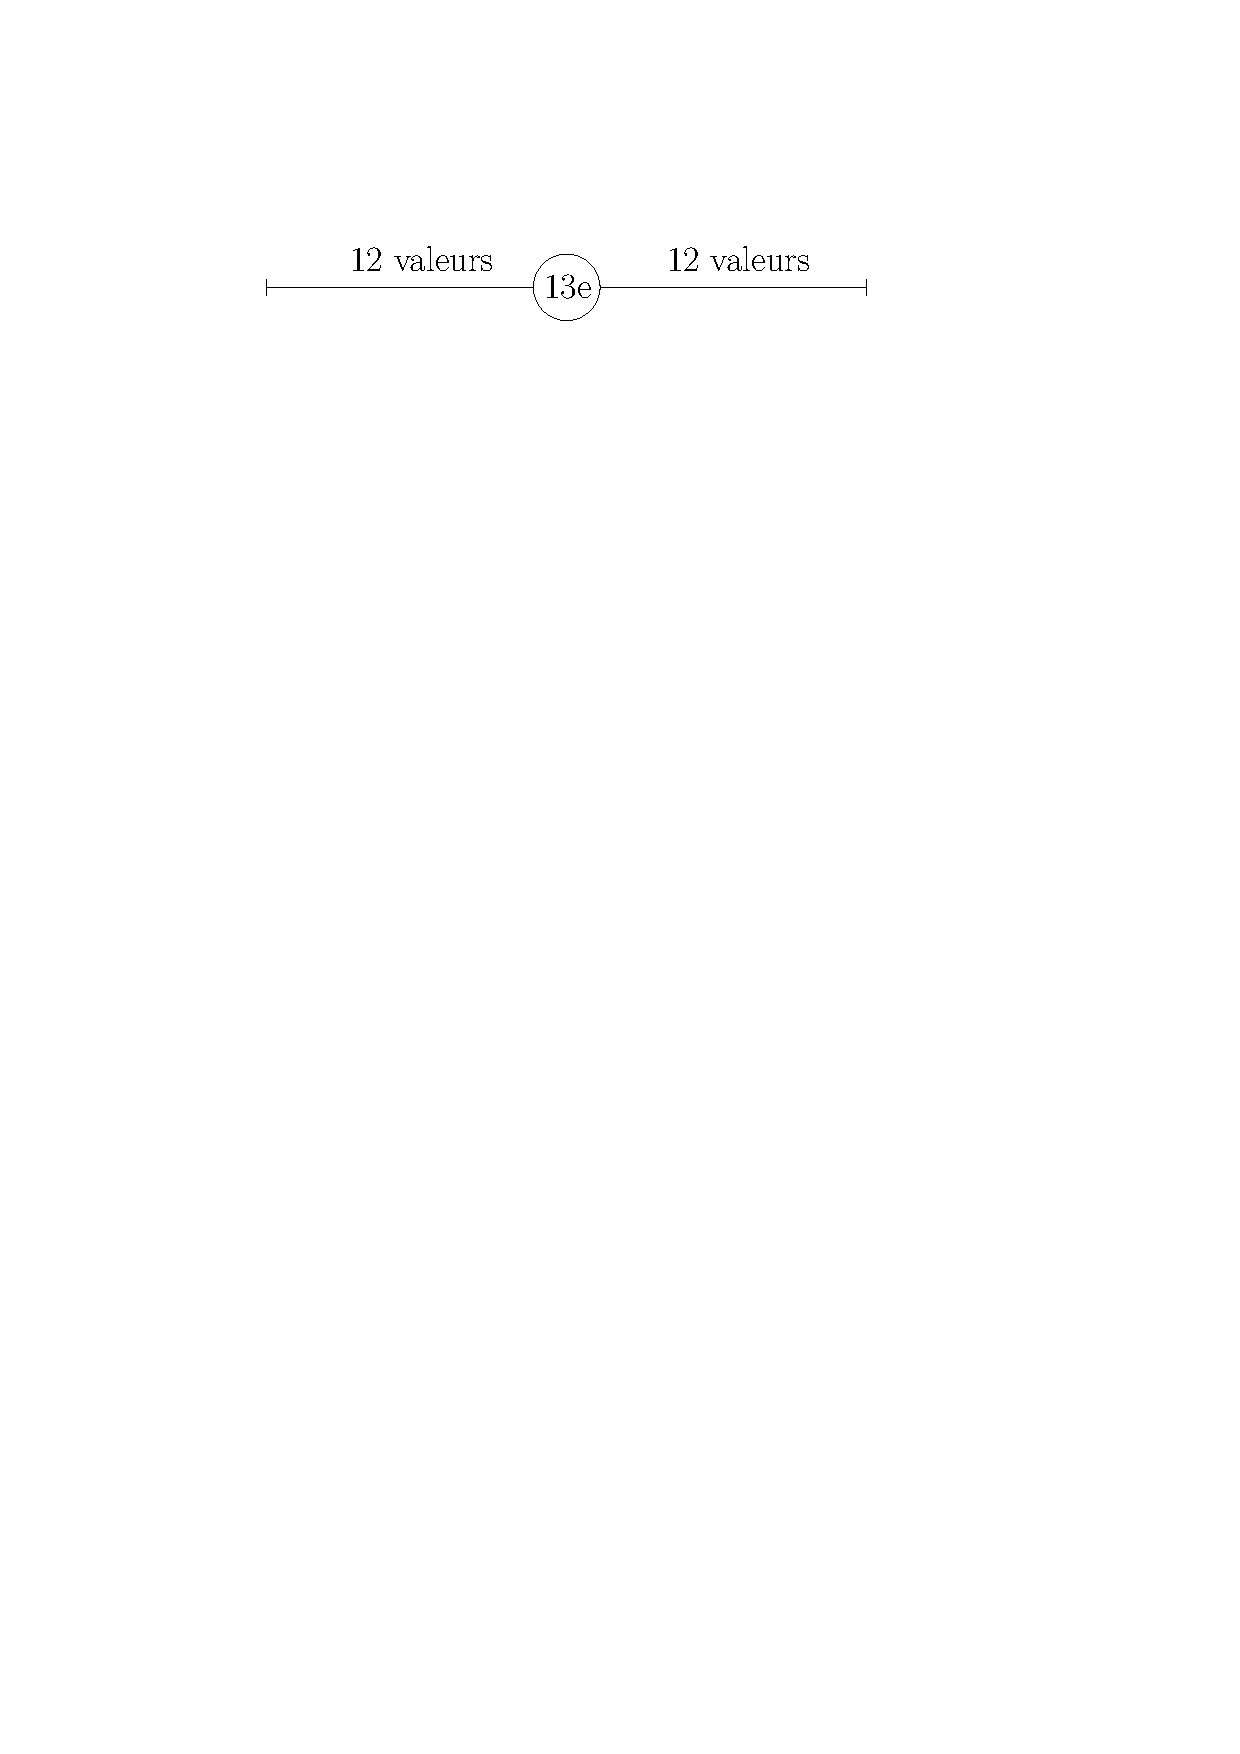
\includegraphics[width=0.6\linewidth]{3xx-dm/sources/dm1/ex1.pdf}
	\end{figure}
	On ordonne la série et on selectionne la treizième valeur.\\
	30 ; 31 ; 31 ; 32 ; 32 ; 33 ; 34 ; 34 ; 36 ; 37 ; 38 ; 38 ; \textbf{39} ; 39 ; 40 ; 40 ; 42 ; 42 ; 43; 43 ; 45 ; 45 ; 46 ; 47 ; 48.\\
	Interprétration :\\
	La médiane de la série de récolte est 39kg. La moité des récoltes sont plus petites que 39kg, l'autre moitié est plus grosse.
	\item[A.c)] Calcul de la moyenne : $\dfrac{\text{somme des valeurs}}{\text{nombre de valeur}}$\\
	moyenne = $\frac{34 + 39 + ... + 47 + 33}{25} = \dfrac{965}{25} \approx 38.6$\\
	La moyenne de la série de récoltes est 38.6 kg.

	\item[B.a)] La brouette est un prisme avec pour base un trapèze.\\
	Aire de base : $A = \dfrac{(B+b)\times h}{2} = \dfrac{(40+70)\times 35}{2} = 1925$\\
	Volume : Aire de base $\times$ hauteur : $V = A \times h = 1925 \times 40 = 77000$\\
	Conversion : $1L = 1dm^3 = 1000cm^3$\\
	$V = 77000 cm^3 = 77 L$\\
	Le volume de la brouette est bien 77L. 
	\item[B.b)]	$900 g = 0.9 kg$.\\
	$77 \times 0.9 = 69.3$.\\
	Le contenu de la brouette de sel pèse : 69.3kg.
\end{itemize}

\end{multicols}
\horrule{1px} 
\begin{multicols}{2}

\subsection*{COURS - Pythagore}
\textit{\textbf{Recopier à l'identique (et apprendre).}}
\paragraph{Théorème de Pythagore}~~\
Si un triangle est rectangle, alors le carré de son plus grand côté est égal à la somme des carrés des deux plus petits côtés.\\
Soit ABC un triangle rectangle en A. Le plus grand côté est en face de l'angle droit donc BC.\\
$BC^2 = AB^2 + AC^2$ 
\paragraph{Modélisation}~~\
\begin{itemize}
	\item Le théorème de Pythagore permet de calculer une longueur dans un triangle rectangle si on connait deux côtés.
	\item La réciproque du théorème de Pythagore permet de démontrer si un triangle est rectangle (ou non) si on connait les trois cotés de ce triangle. 
\end{itemize}
\end{multicols}

\horrule{1px} 

\begin{multicols}{2}

\subsection*{Ex - Pythagore}
\textit{\textbf{Faire les trois questions.}}
\begin{itemize}
\item[1.] Soit NAC un triangle rectangle en A tel que : NA = 12 cm et CA = 5 cm.\\
Calculer la longueur NC.
\item[2.] Soit TNJ un triangle rectangle en J tel que : NJ = 8,4 cm et TN = 14 cm.\\
Calculer la longueur TJ.
\item[3.] Soit JEL un triangle tel que : EL = 17,8 cm, EJ = 16 cm et LJ = 7,8 cm.\\
Quelle est la nature du triangle JEL ?
\end{itemize}

\end{multicols}
\horrule{1px} 
\begin{multicols}{2}

\subsection*{Ex - Résoudre}
\textit{\textbf{Résoudre les équations.}}
\begin{itemize}
\item[1.] $2x = 80 $
\item[2.] $x + 24 = 144 $
\item[3.] $x - 30 = 42 $
\item[4.] $2x + 8 = 100 $
\item[5.] $100 - x = 32$
\item[6.] $6x + 10 = 4x + 20$
\end{itemize}

\end{multicols}

\end{document}